In order to state the interaction between the different components of the system here are presented some sequence diagrams.
\\The sequence diagrams highlight the part of the system that interact for implement a function and the messages exchanged between them.


\begin{figure}[!ht]
  \centering
  \vspace{0.2cm}
  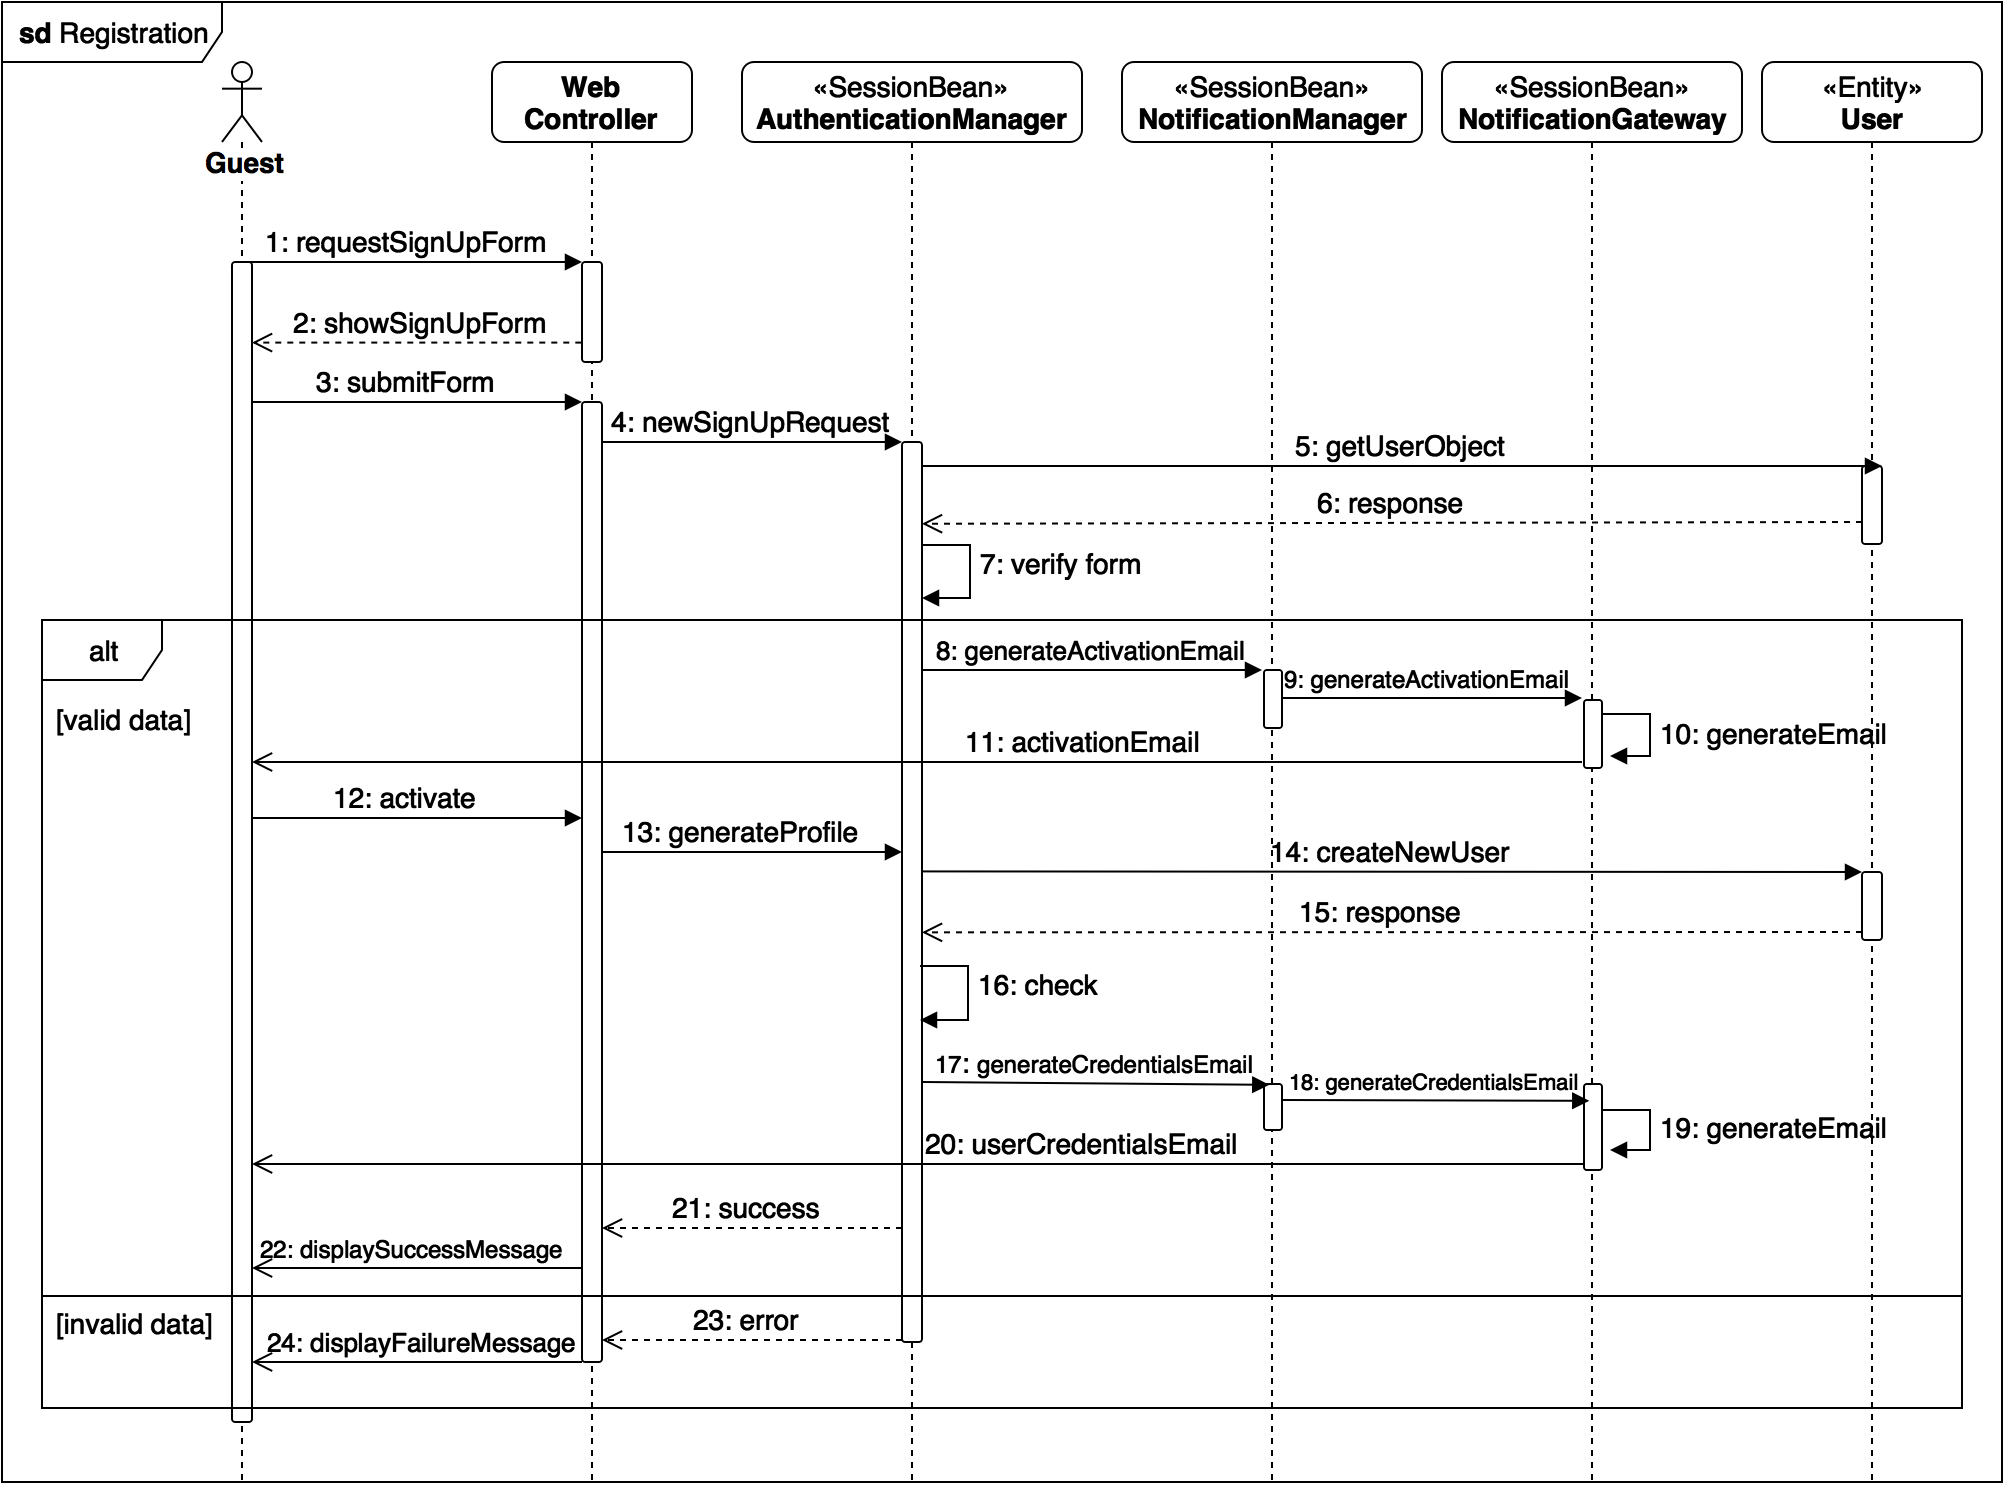
\includegraphics[width=1.15\textwidth, angle=90]{/DD/registration_runtime}\\
  \vspace{0.4cm}
  \caption{Sequence diagram for the registration process using the web application.} 
  \label{fig:registration_runtime} 
\end{figure}
\newpage
\begin{figure}[!ht]
  \centering
  \vspace{0.2cm}
  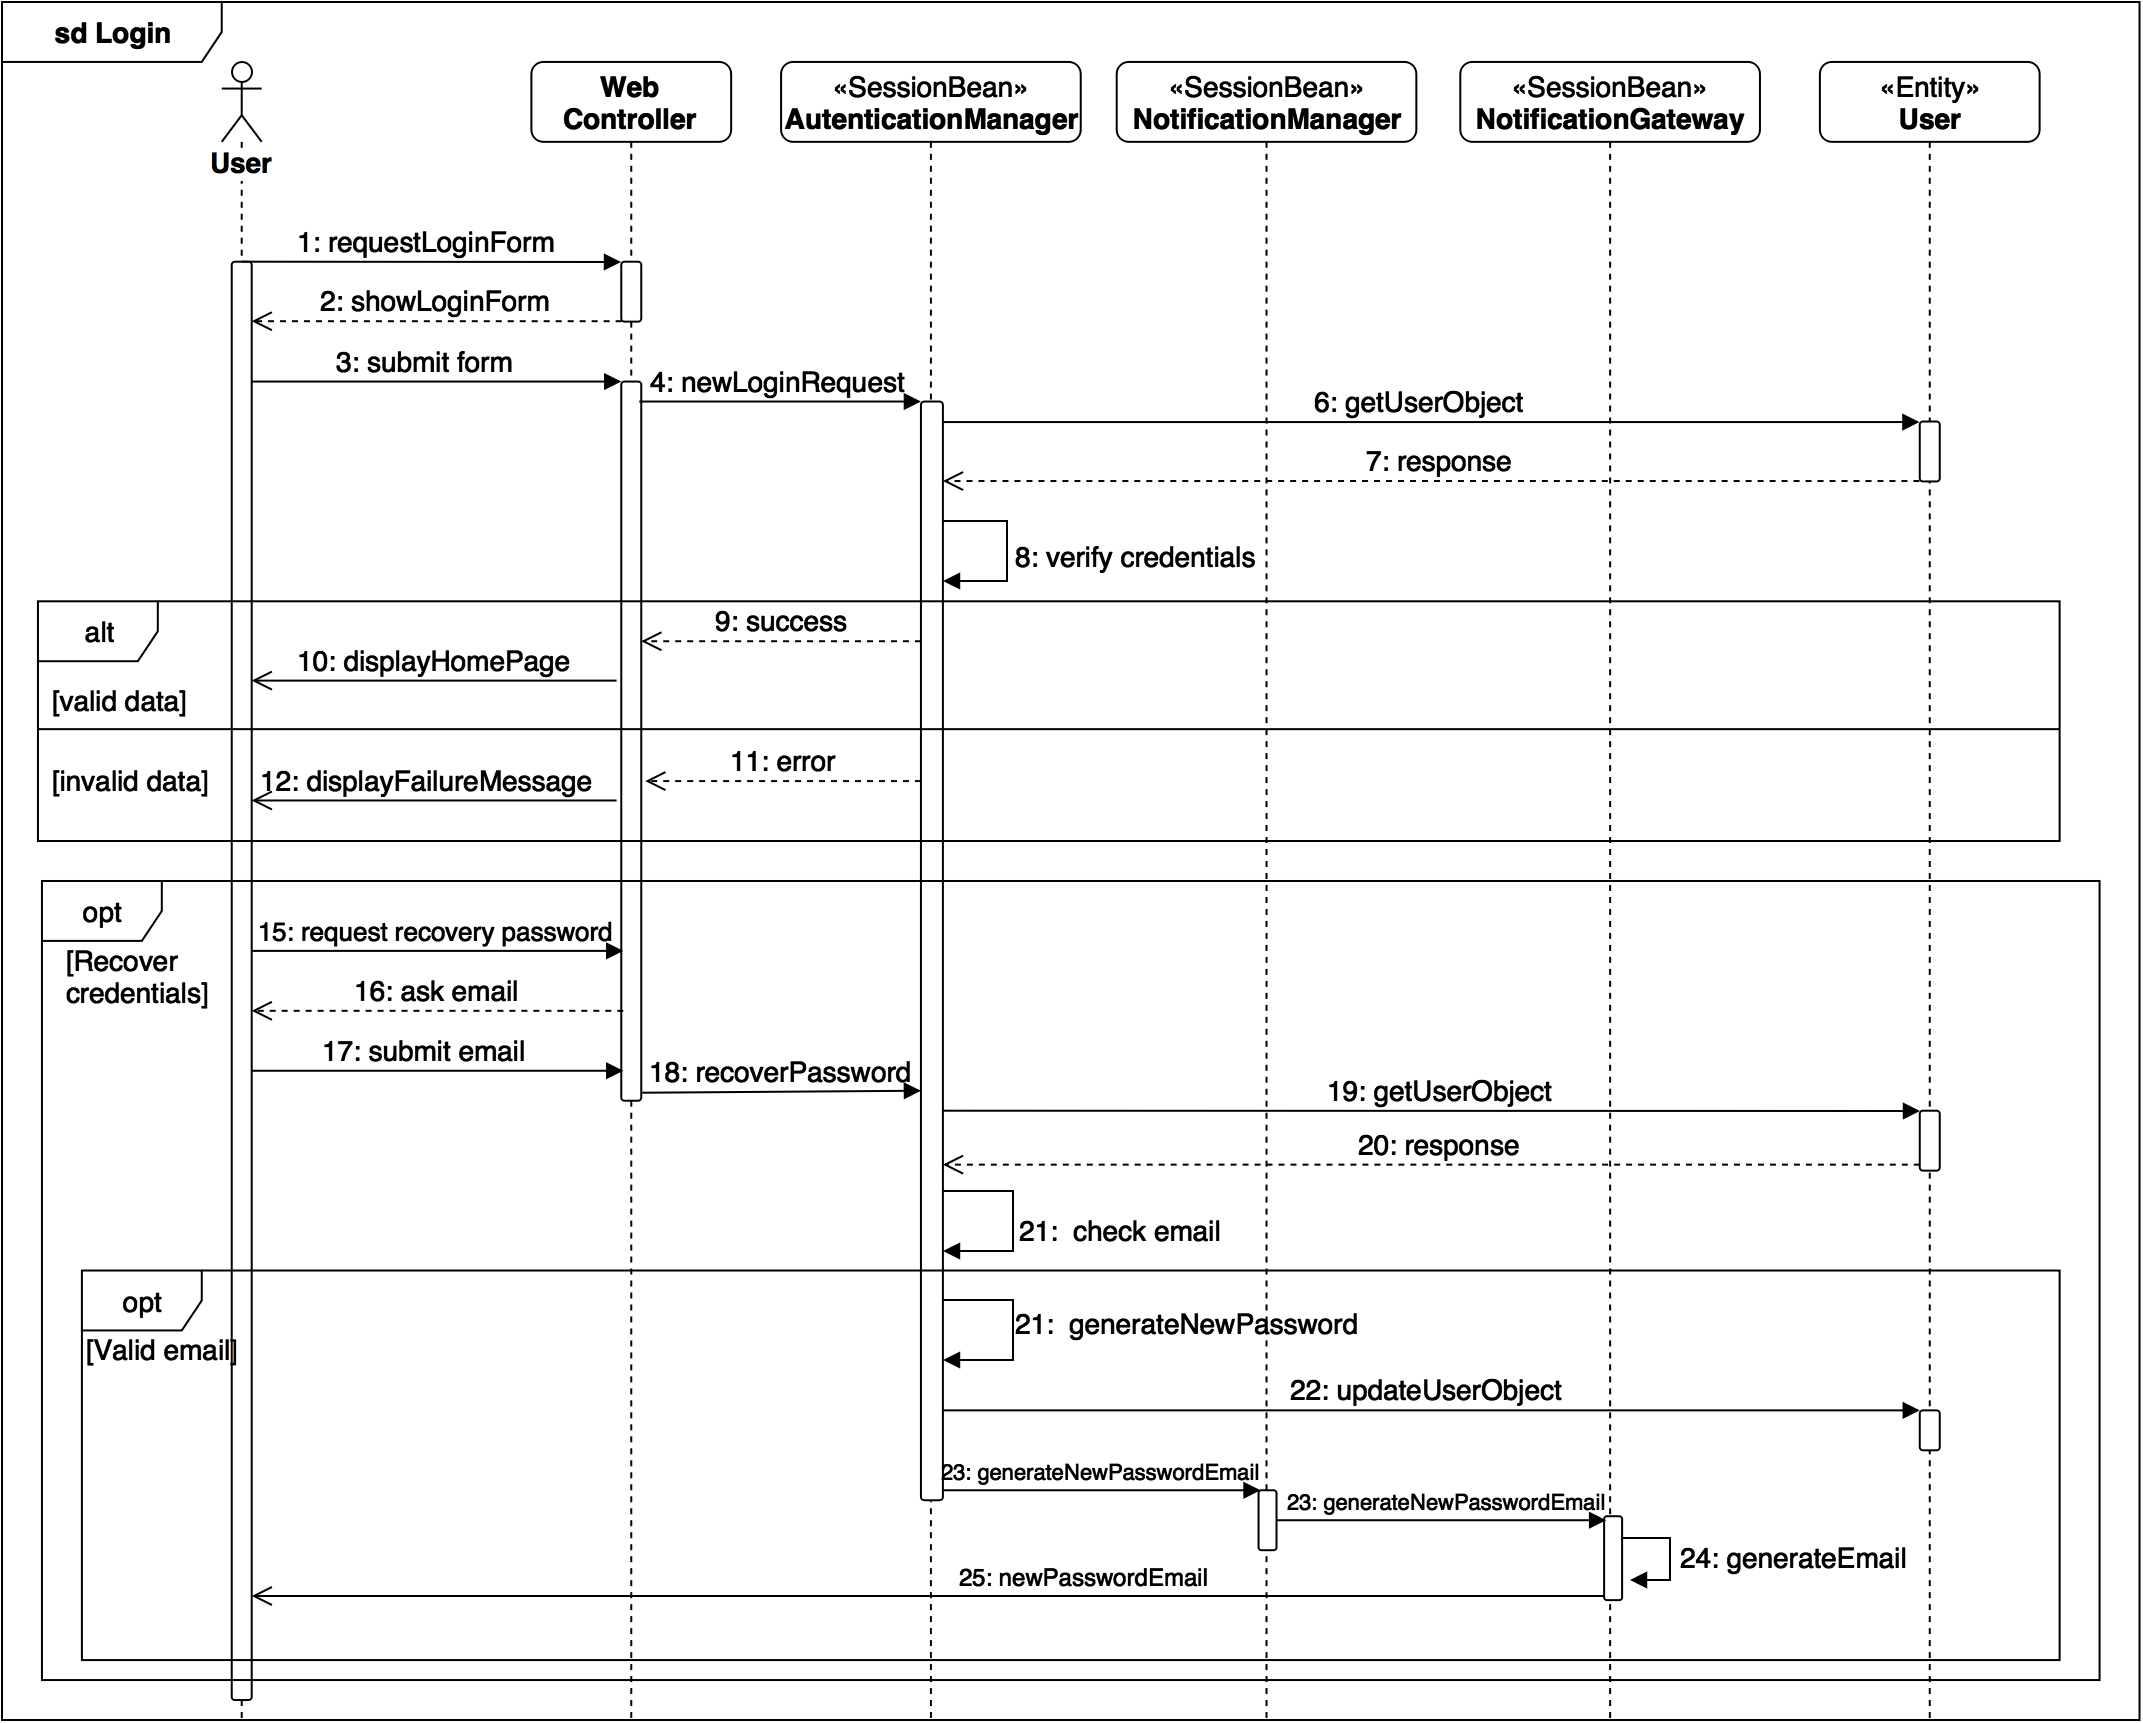
\includegraphics[width=1.4\textwidth, angle=90]{/DD/login_runtime}\\
  \vspace{0.4cm}
  \caption{Sequence diagram for the login process using the web application.} 
  \label{fig:login_runtime} 
\end{figure}
\newpage
\begin{figure}[!ht]
  \centering
  \vspace{0.2cm}
  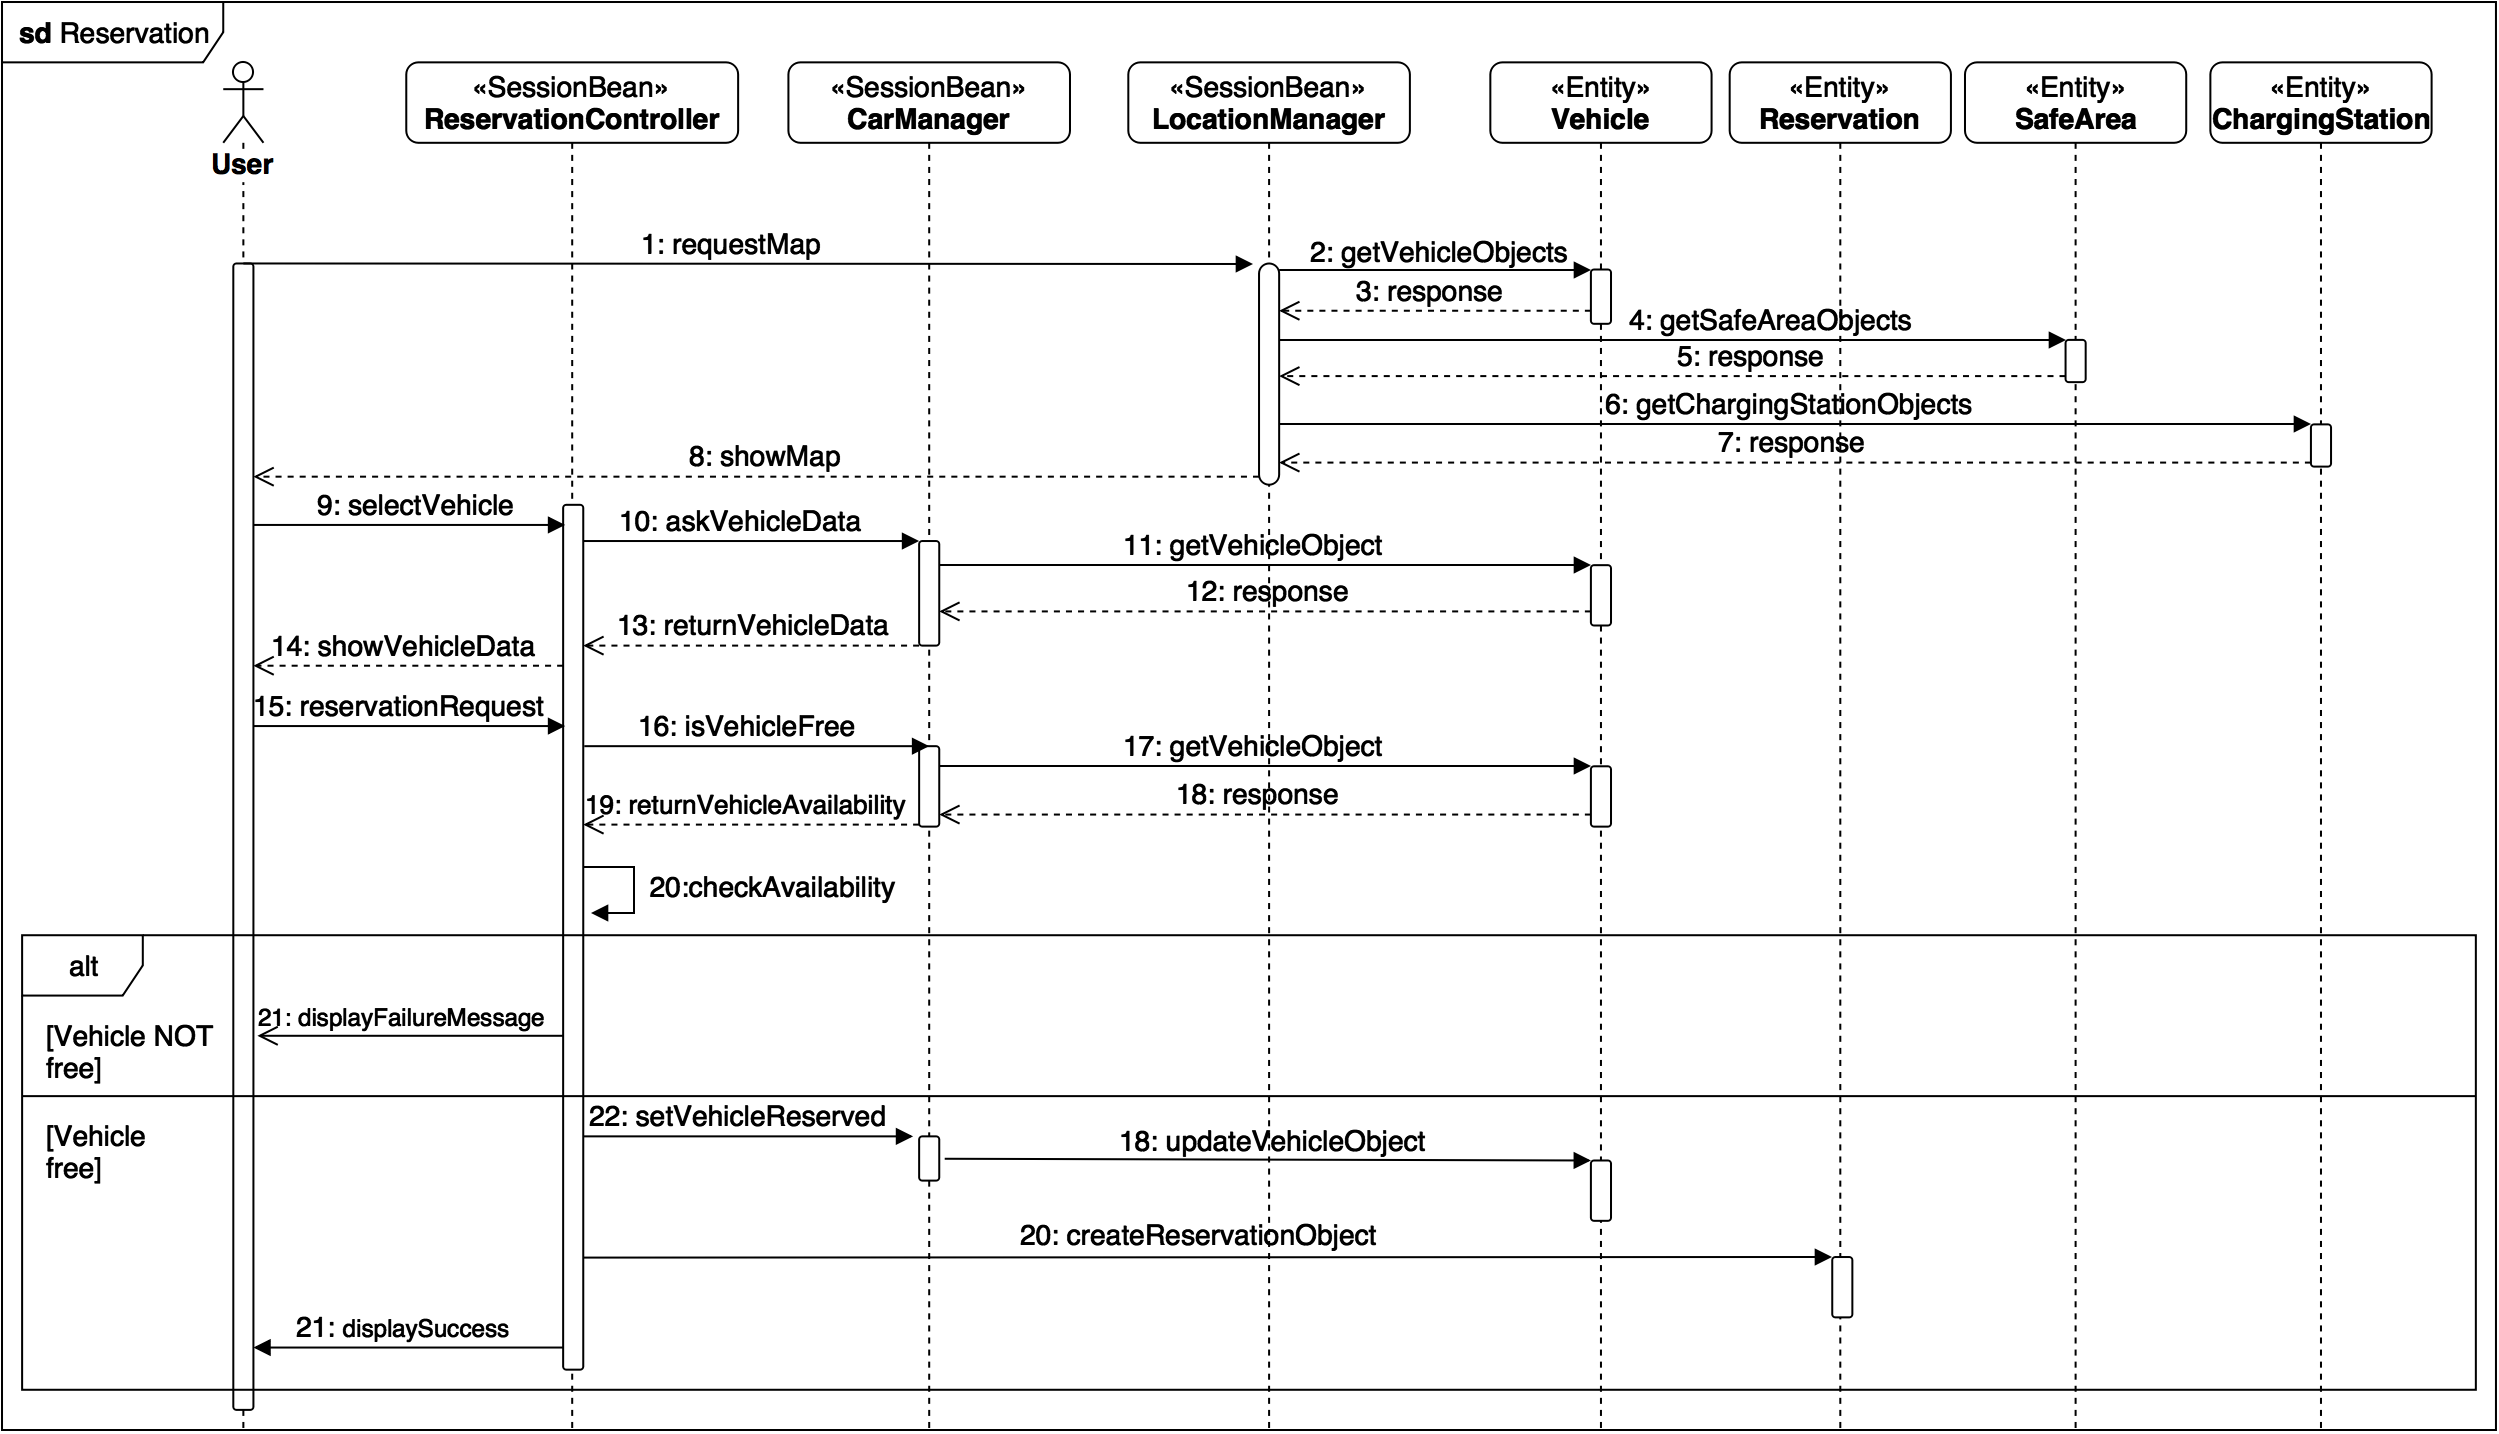
\includegraphics[width=1.4\textwidth, angle=90]{/DD/reservation_runtime}\\
  \vspace{0.4cm}
  \caption{Sequence diagram for the reservation process using the mobile application.} 
  \label{fig:reservation_runtime} 
\end{figure}
\newpage
\begin{figure}[!ht]
  \centering
  \vspace{0.2cm}
  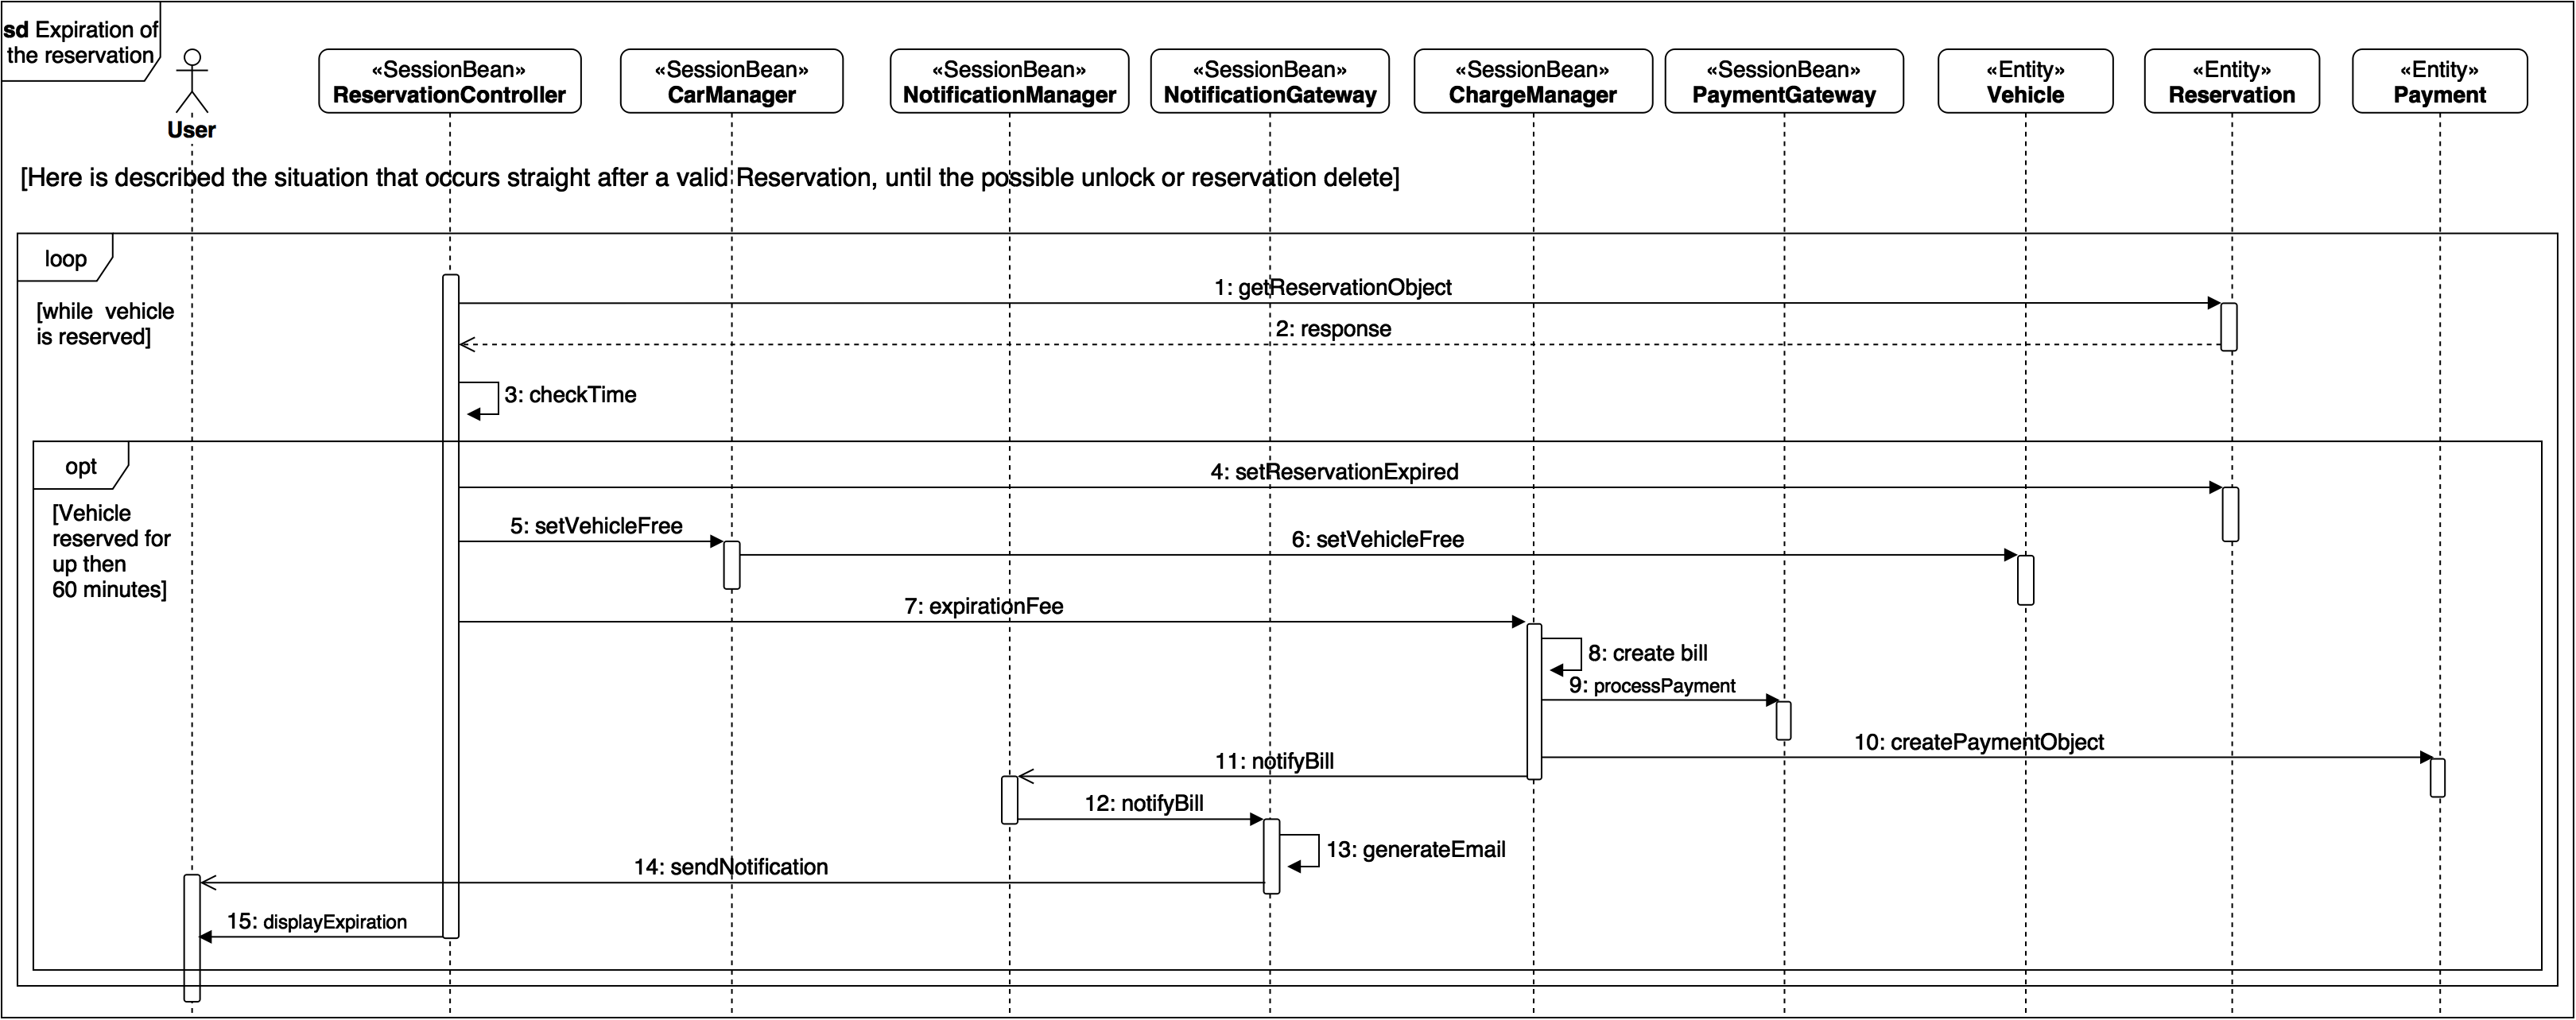
\includegraphics[width=1.4\textwidth, angle=90]{/DD/expiration_runtime}\\
  \vspace{0.4cm}
  \caption{Sequence diagram for the reservation's expiration.} 
  \label{fig:expiration_runtime} 
\end{figure}
\newpage
\begin{figure}[!ht]
  \centering
  \vspace{0.2cm}
  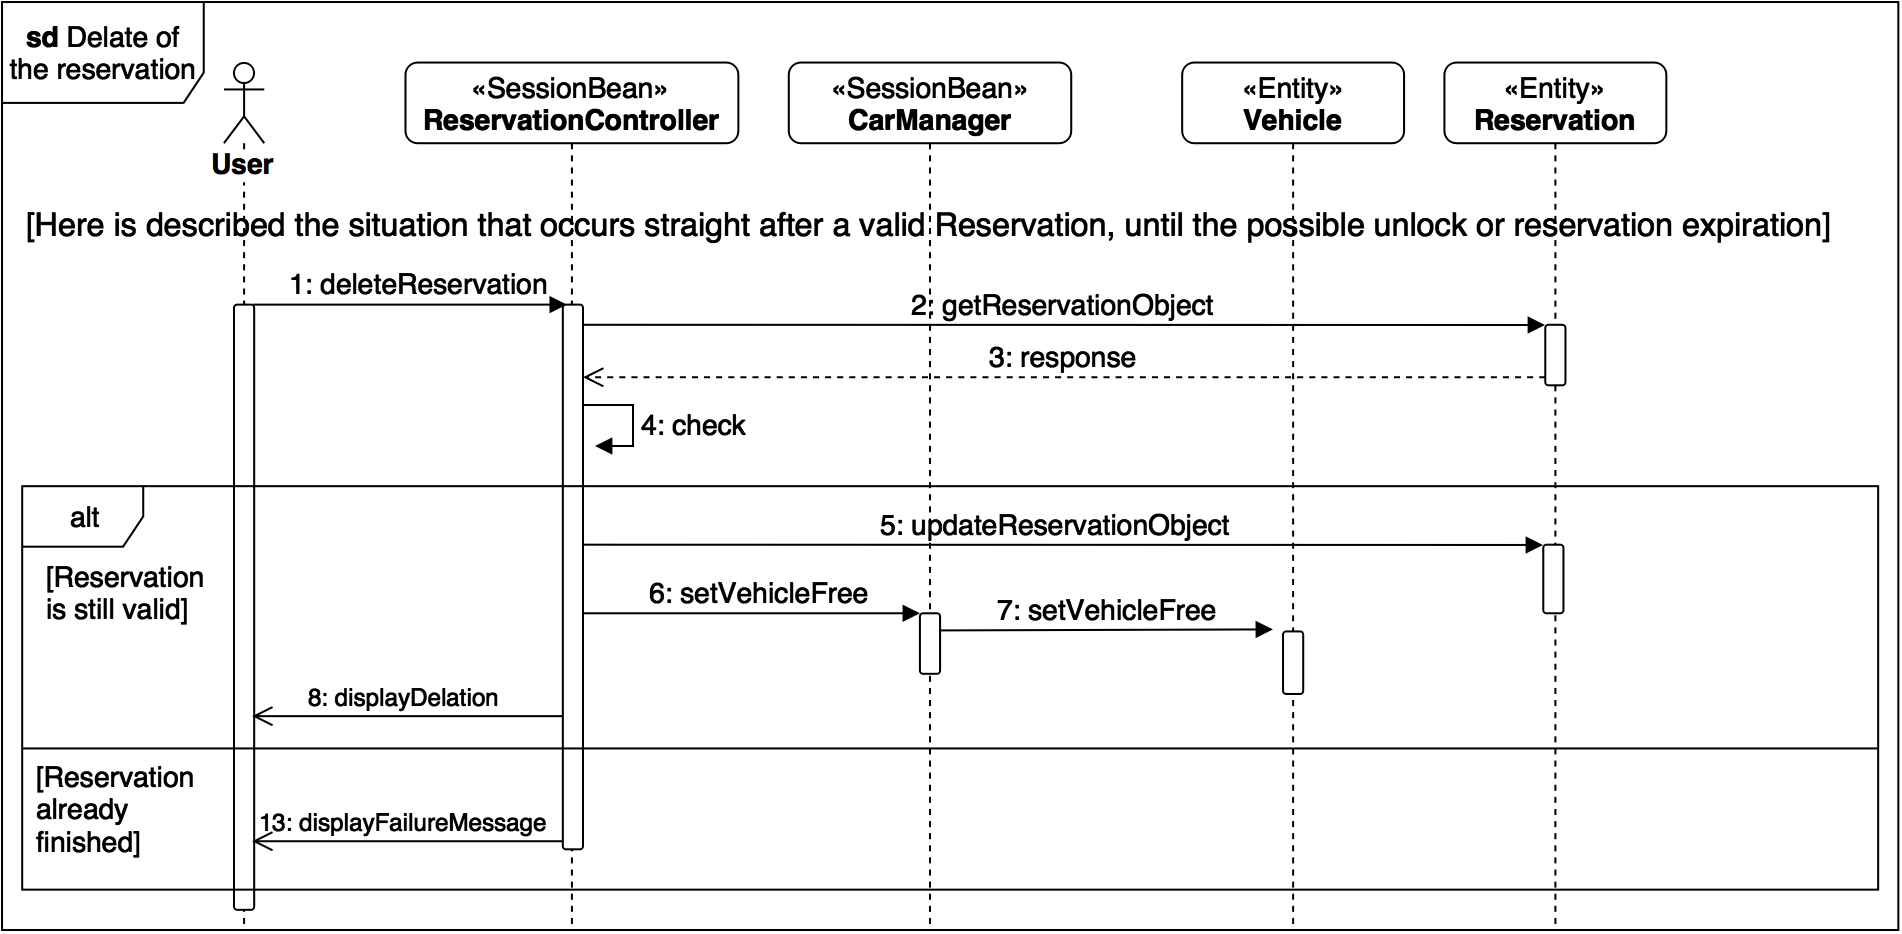
\includegraphics[width=1.4\textwidth, angle=90]{/DD/delete_reservation_runtime}\\
  \vspace{0.4cm}
  \caption{Sequence diagram for the reservation's deletion using the mobile application.} 
  \label{fig:delete_reservation_runtime} 
\end{figure}
\newpage
\begin{figure}[!ht]
  \centering
  \vspace{0.2cm}
  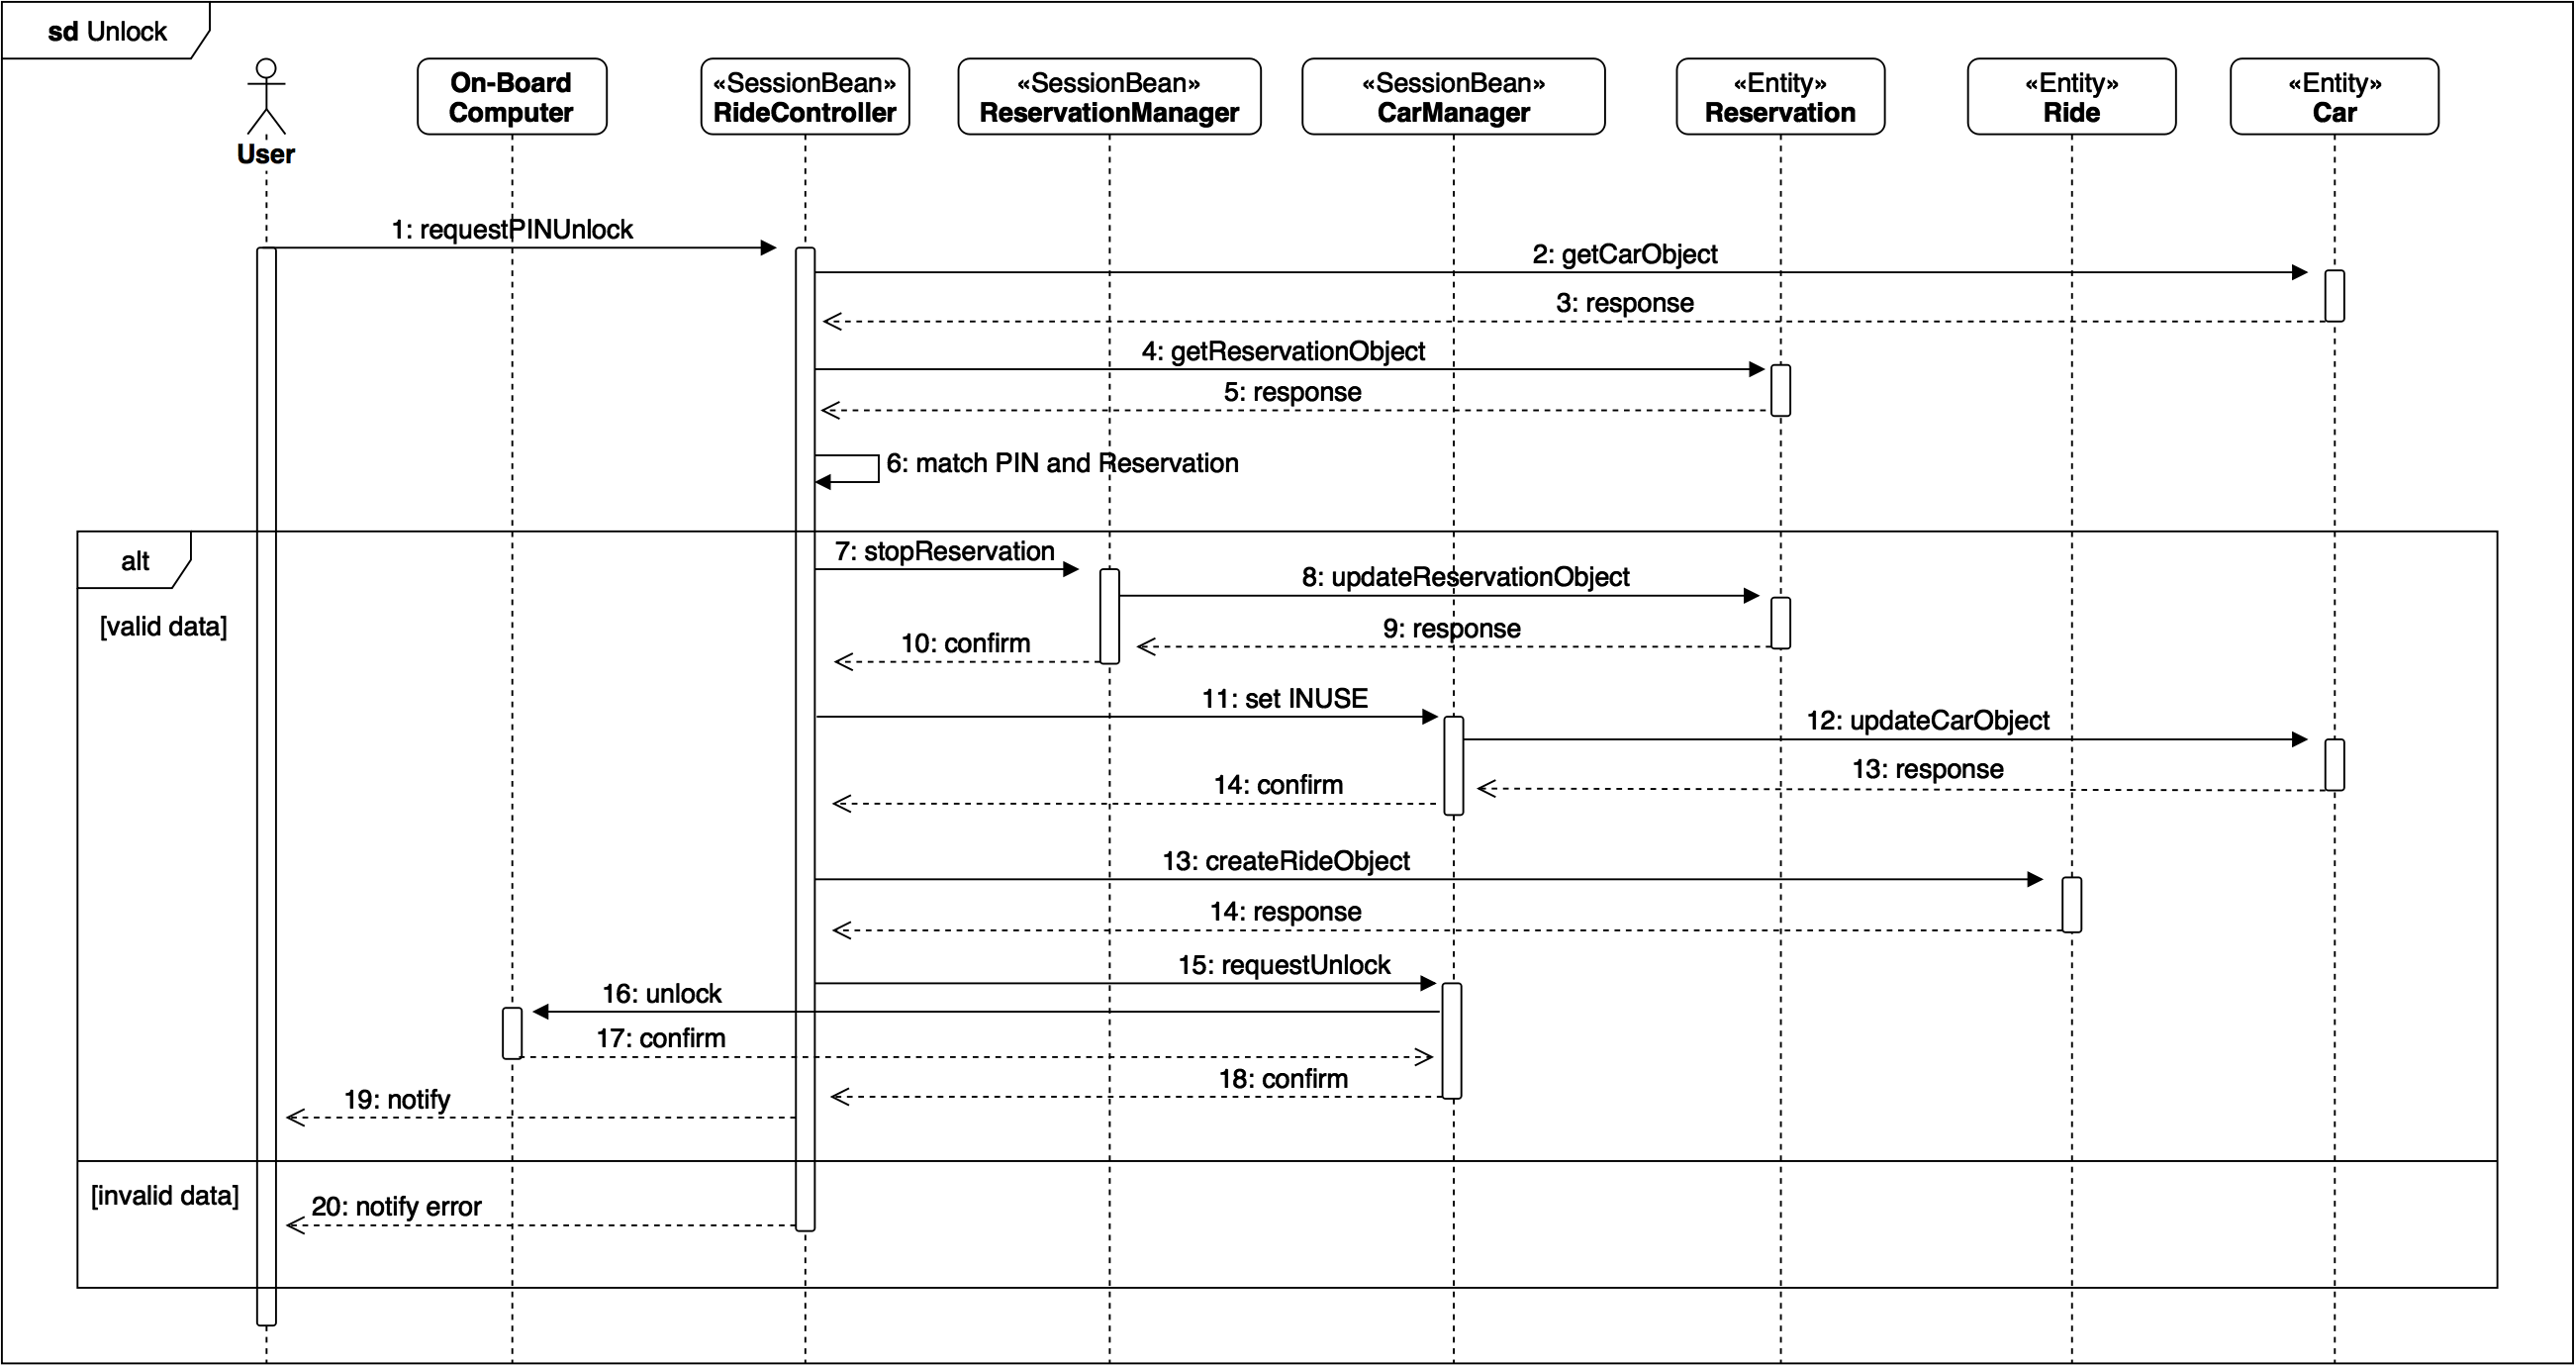
\includegraphics[width=1.4\textwidth, angle=90]{/DD/unlock_runtime}\\
  \vspace{0.4cm}
  \caption{Sequence diagram for the car un-lock process. The unlockRequest (as specified in the RASD document) must contain the car's PIN code.} 
  \label{fig:unlock_runtime} 
\end{figure}
\newpage
\begin{figure}[!ht]
  \centering
  \vspace{0.2cm}
  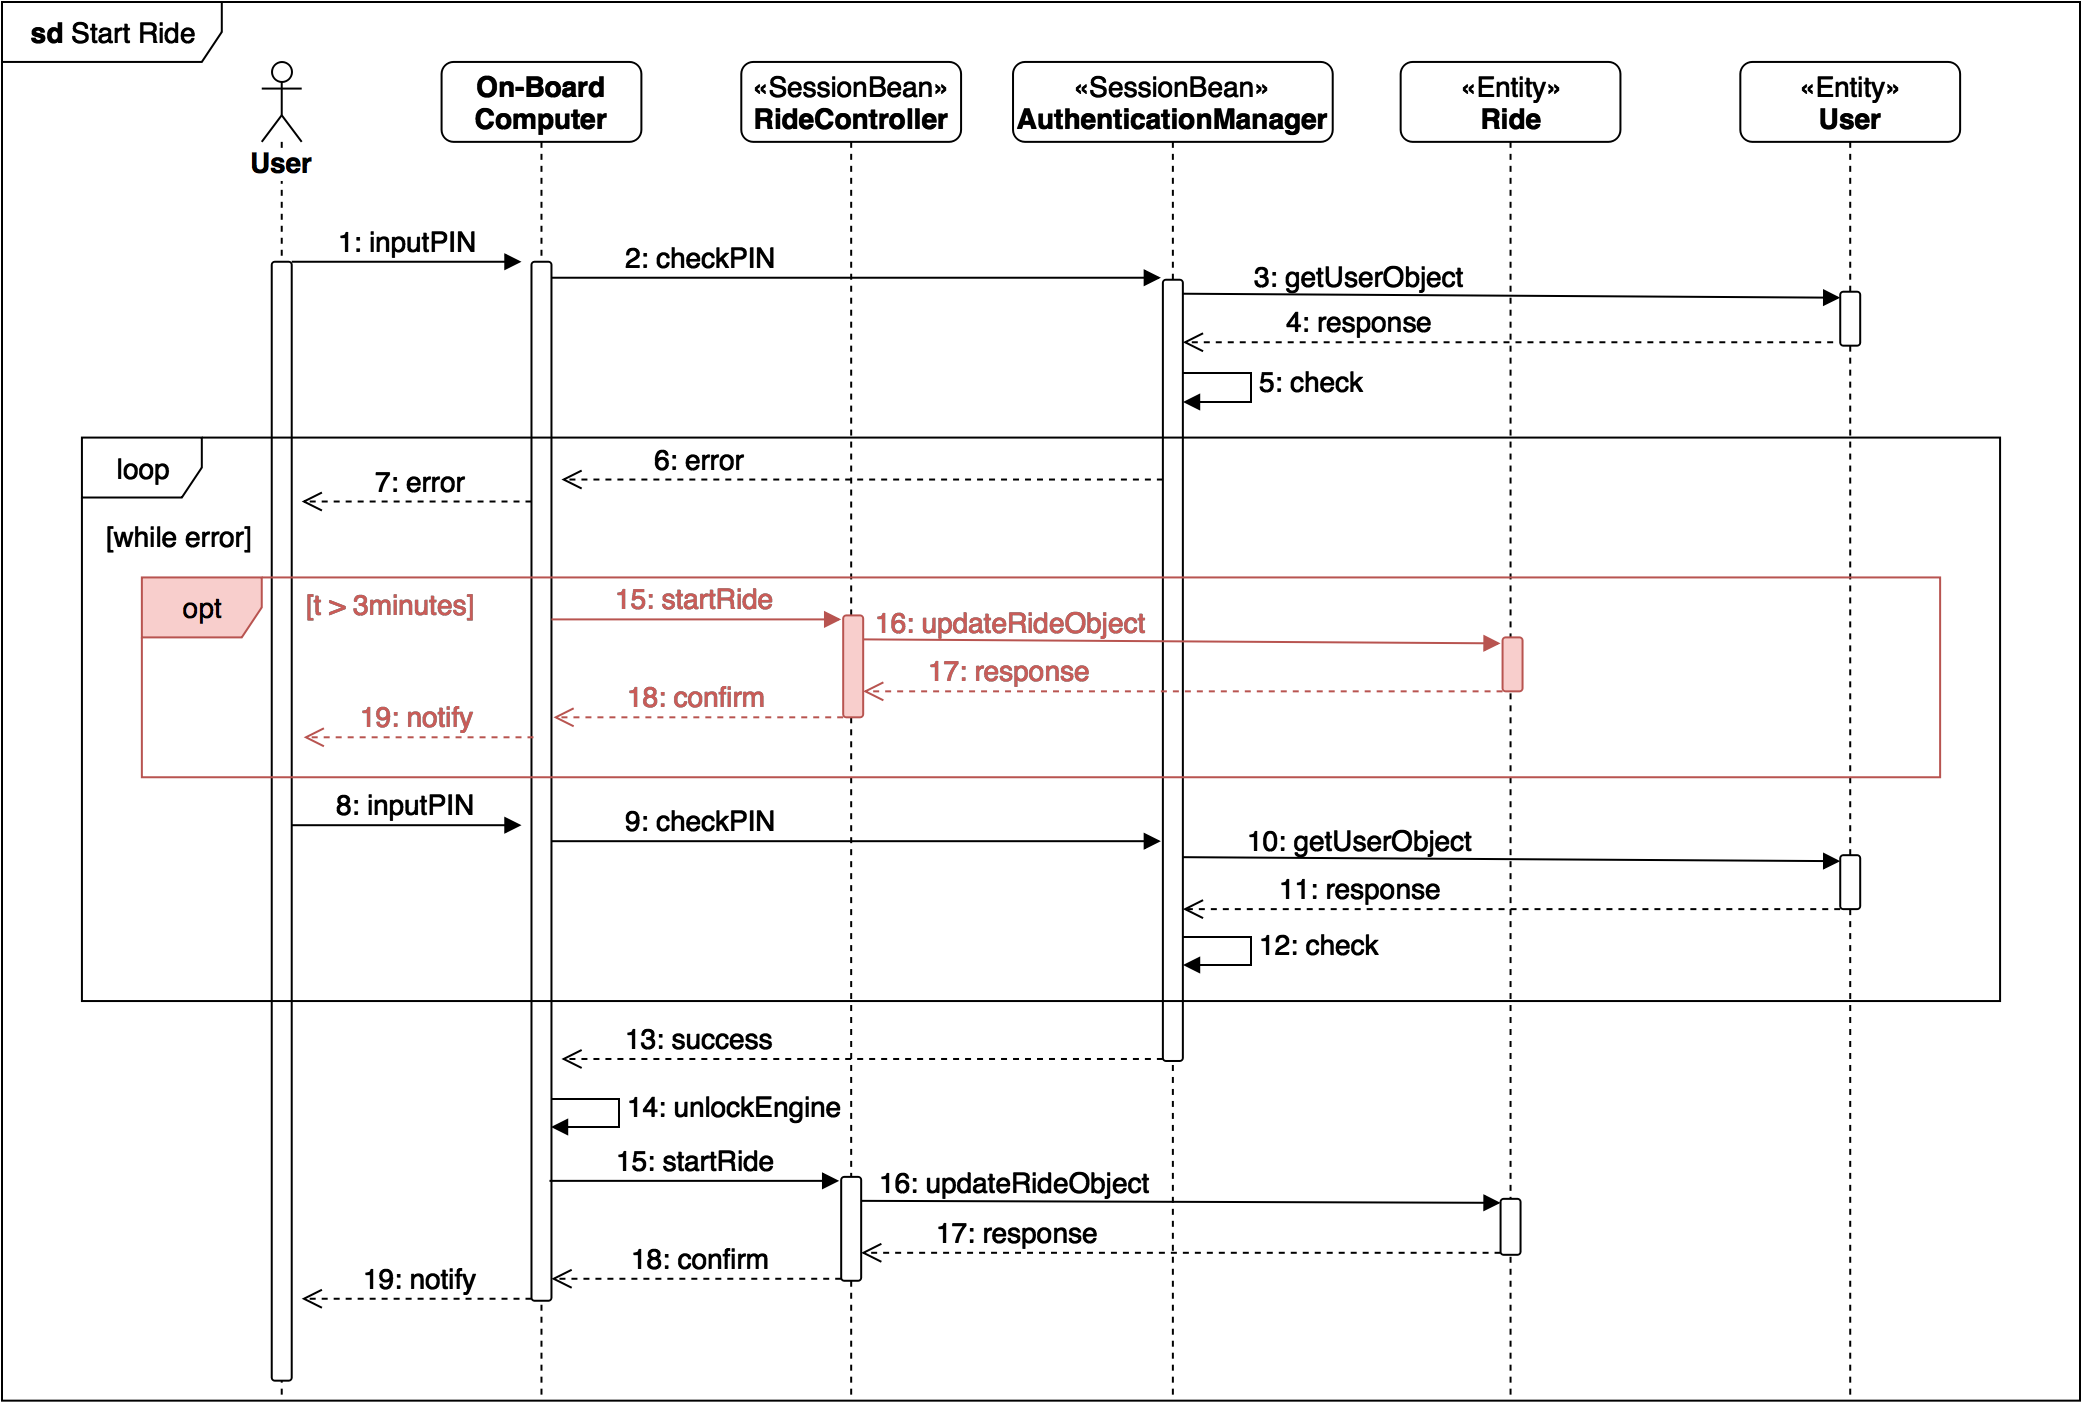
\includegraphics[width=1.35\textwidth, angle=90]{/DD/start_runtime}\\
  \vspace{0.4cm}
  \caption{Sequence diagram for the start-ride process. It is important to highlight an abuse of terminology: the PIN keyword is used here representing the car-code (which is visible on the vehicle's windscreen) and in \ref{fig:unlock_runtime} representing the user's personal code.}
  \label{fig:start_runtime} 
\end{figure}
\newpage
\begin{figure}[!ht]
  \centering
  \vspace{0.2cm}
  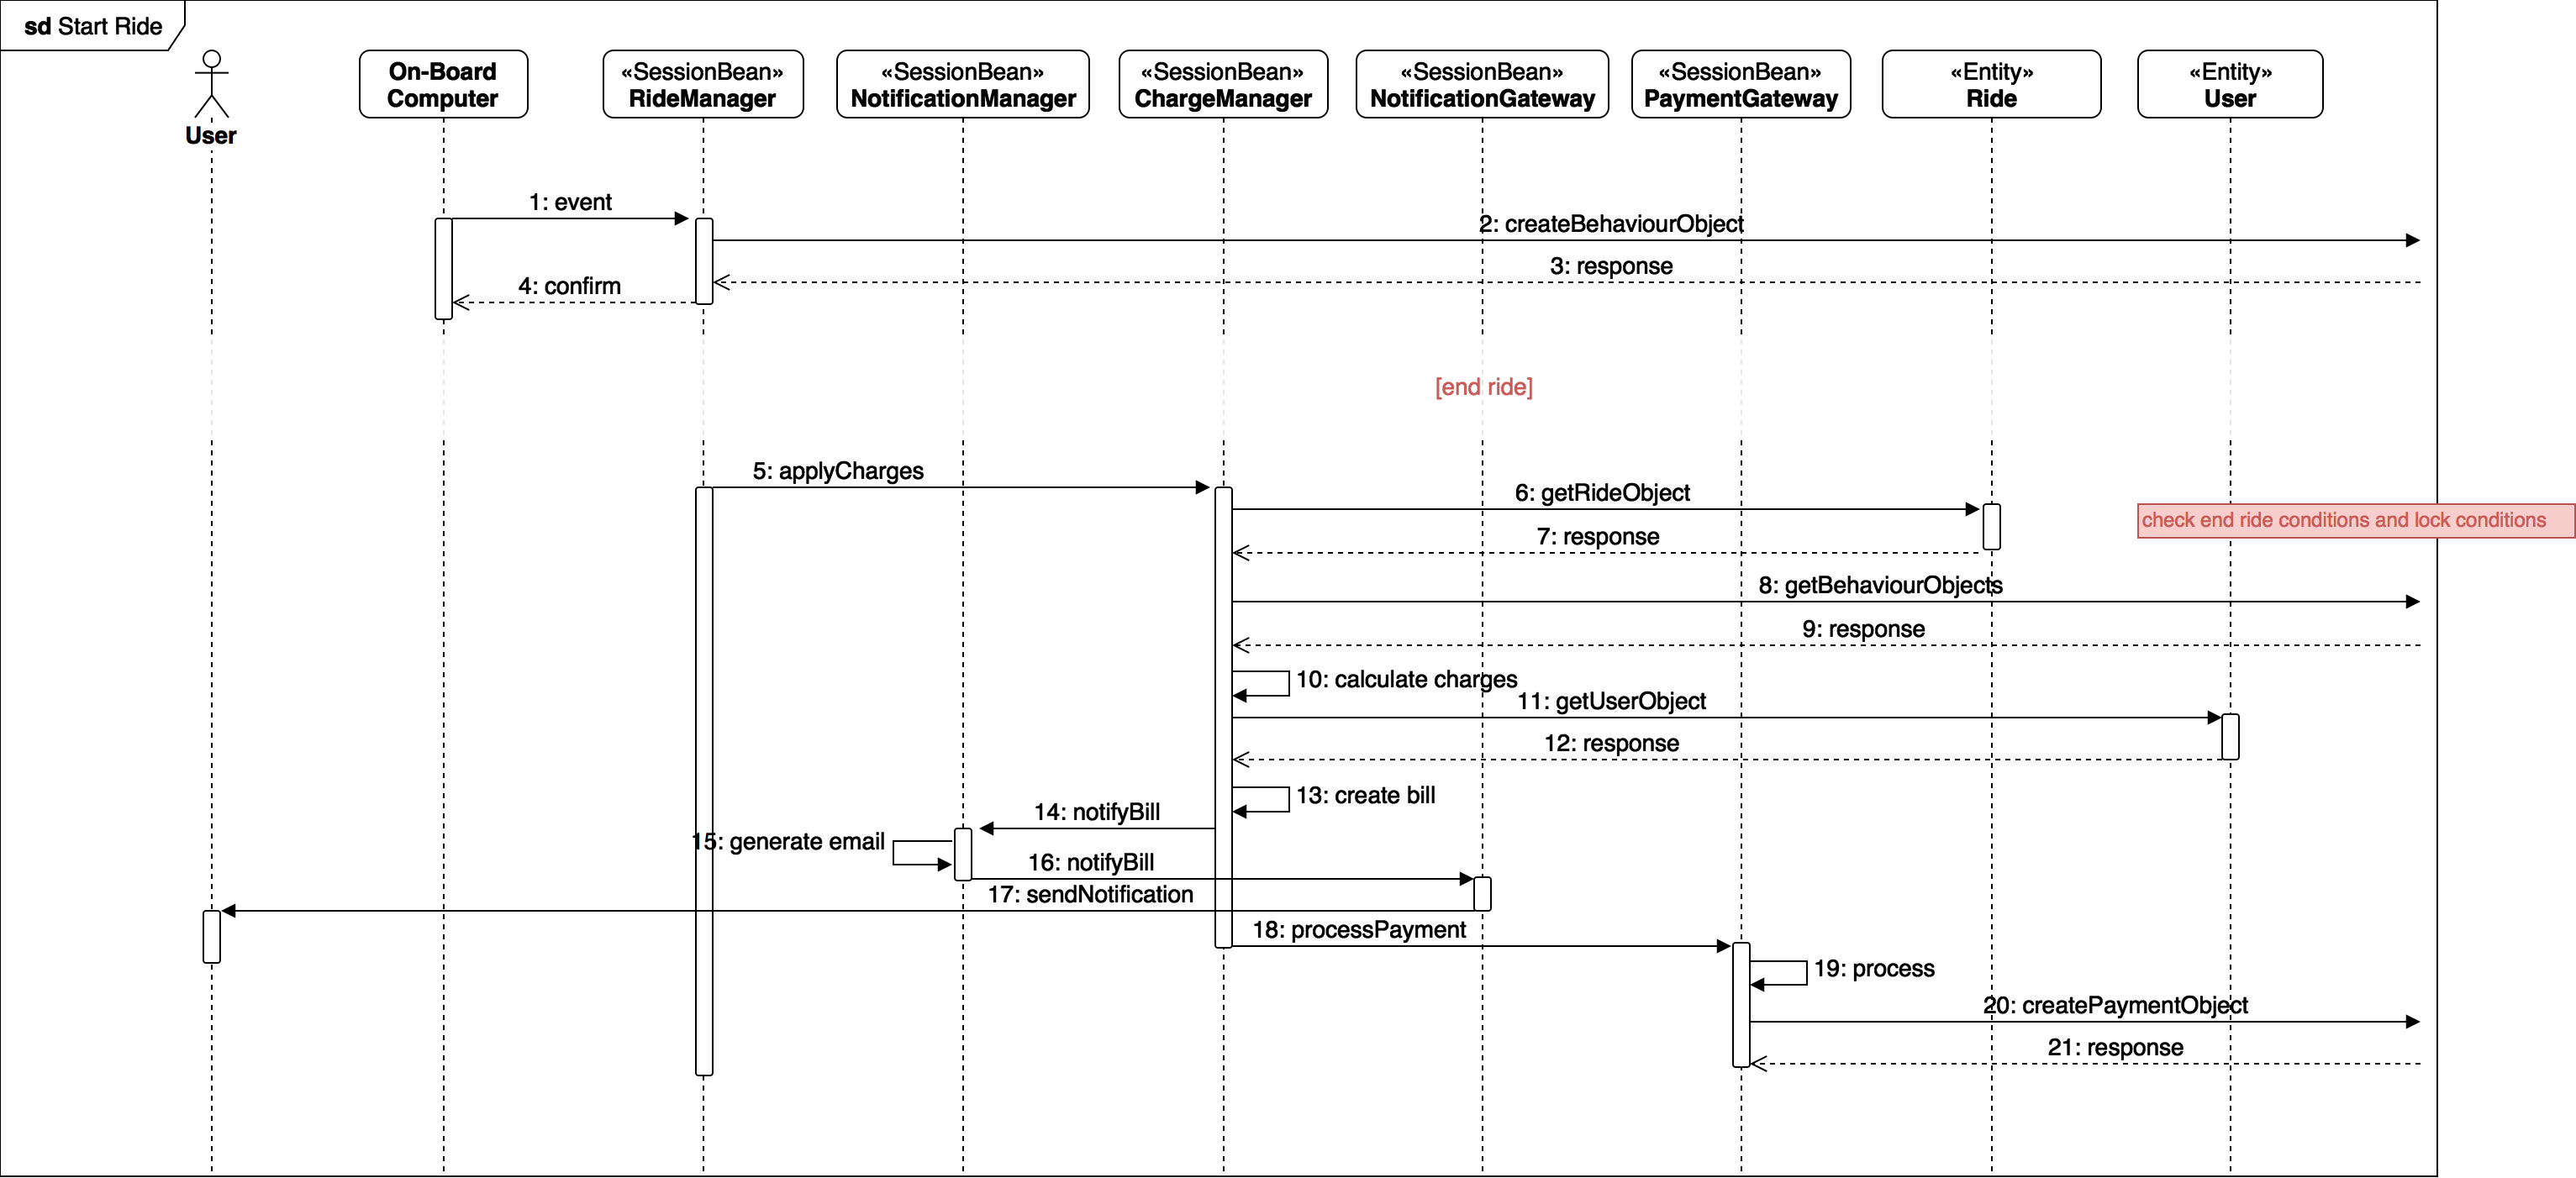
\includegraphics[width=1.4\textwidth, angle=90]{/DD/charge_runtime}\\
  \vspace{0.4cm}
  \caption{Sequence diagram for the charges computation and application. We decided to use an event-driven approach for the behaviour detection.} 
  \label{fig:charge_runtime} 
\end{figure}
\newpage